
\documentclass[conference]{IEEEtran}
% *** CITATION PACKAGES ***
%\usepackage{cite}

% *** GRAPHICS RELATED PACKAGES ***
\ifCLASSINFOpdf
   \usepackage[pdftex]{graphicx}
\else
  \usepackage[dvips]{graphicx}
\fi

% *** MATH PACKAGES ***
\usepackage[cmex10]{amsmath}
\newcommand{\argmin}{\operatornamewithlimits{argmin}}

% *** SPECIALIZED LIST PACKAGES ***
\usepackage{algorithm}
\usepackage{algpseudocode}


% *** ALIGNMENT PACKAGES ***
%\usepackage{array}

%\usepackage{mdwmath}
%\usepackage{mdwtab}
% Also highly recommended is Mark Wooding's extremely powerful MDW tools,
% especially mdwmath.sty and mdwtab.sty which are used to format equations
% and tables, respectively. The MDWtools set is already installed on most
% LaTeX systems. The lastest version and documentation is available at:
% http://www.ctan.org/tex-archive/macros/latex/contrib/mdwtools/


% IEEEtran contains the IEEEeqnarray family of commands that can be used to
% generate multiline equations as well as matrices, tables, etc., of high
% quality.


%\usepackage{eqparbox}
% Also of notable interest is Scott Pakin's eqparbox package for creating
% (automatically sized) equal width boxes - aka "natural width parboxes".
% Available at:
% http://www.ctan.org/tex-archive/macros/latex/contrib/eqparbox/


% *** SUBFIGURE PACKAGES ***
\usepackage[caption=false]{caption}
\usepackage[font=footnotesize]{subfig}
% subfig.sty, also written by Steven Douglas Cochran, is the modern
% replacement for subfigure.sty. However, subfig.sty requires and
% automatically loads Axel Sommerfeldt's caption.sty which will override
% IEEEtran.cls handling of captions and this will result in nonIEEE style
% figure/table captions. To prevent this problem, be sure and preload
% caption.sty with its "caption=false" package option. This is will preserve
% IEEEtran.cls handing of captions. Version 1.3 (2005/06/28) and later 
% (recommended due to many improvements over 1.2) of subfig.sty supports
% the caption=false option directly:
%\usepackage[caption=false,font=footnotesize]{subfig}
%
% The latest version and documentation can be obtained at:
% http://www.ctan.org/tex-archive/macros/latex/contrib/subfig/
% The latest version and documentation of caption.sty can be obtained at:
% http://www.ctan.org/tex-archive/macros/latex/contrib/caption/




% *** FLOAT PACKAGES ***
%
%\usepackage{fixltx2e}
% fixltx2e, the successor to the earlier fix2col.sty, was written by
% Frank Mittelbach and David Carlisle. This package corrects a few problems
% in the LaTeX2e kernel, the most notable of which is that in current
% LaTeX2e releases, the ordering of single and double column floats is not
% guaranteed to be preserved. Thus, an unpatched LaTeX2e can allow a
% single column figure to be placed prior to an earlier double column
% figure. The latest version and documentation can be found at:
% http://www.ctan.org/tex-archive/macros/latex/base/



%\usepackage{stfloats}
% stfloats.sty was written by Sigitas Tolusis. This package gives LaTeX2e
% the ability to do double column floats at the bottom of the page as well
% as the top. (e.g., "\begin{figure*}[!b]" is not normally possible in
% LaTeX2e). It also provides a command:
%\fnbelowfloat
% to enable the placement of footnotes below bottom floats (the standard
% LaTeX2e kernel puts them above bottom floats). This is an invasive package
% which rewrites many portions of the LaTeX2e float routines. It may not work
% with other packages that modify the LaTeX2e float routines. The latest
% version and documentation can be obtained at:
% http://www.ctan.org/tex-archive/macros/latex/contrib/sttools/
% Documentation is contained in the stfloats.sty comments as well as in the
% presfull.pdf file. Do not use the stfloats baselinefloat ability as IEEE
% does not allow \baselineskip to stretch. Authors submitting work to the
% IEEE should note that IEEE rarely uses double column equations and
% that authors should try to avoid such use. Do not be tempted to use the
% cuted.sty or midfloat.sty packages (also by Sigitas Tolusis) as IEEE does
% not format its papers in such ways.

\begin{document}
\title{A Randomized Planner for Trajectory-Wide Visibility Constraints}

% author names and affiliations
% use a multiple column layout for up to three different
% affiliations
\author{\IEEEauthorblockN{Matthew Klingensmith}
\IEEEauthorblockA{The Robotics Institute\\
Carnegie Mellon University\\
}}

% make the title area
\maketitle


\begin{abstract}
-
\end{abstract}

\IEEEpeerreviewmaketitle

\newcommand{\R}{\mathbf{R}}
\newcommand{\Cfree}{C_{\text{free}}}
\newcommand{\Cobs}{C_{\text{obs}}}
\newcommand{\qinit}{q_{\text{init}}}
\newcommand{\qfinal}{q_{\text{final}}}
\newcommand{\vis}{\textsc{Visible}}
\newcommand{\cfree}{\textsc{Free}}

\section{Problem Sketch}

Consider a robot with one or more sensors mounted on it.  How do we move the
robot such that it can see unknown obstacles and avoid them before hitting them?

The robot has an $N$-dimensional configuration space $C \subseteq \R^{N}$. Parts
of the configuration space either do not intersect obstacles: $\Cfree \subseteq C$,
or else intersect them: $\Cobs \subseteq C$. 

The classical motion planning task is to find a trajectory from an initial
configuration $\qinit \in \Cfree$, to a final configuration $\qfinal \in
\Cfree$ such that all the configurations are in the free space (a condition
called \cfree):

\begin{equation}
\xi =\{ \qinit, q_1, \ldots, \qfinal \} \text{s.t~} \forall q \in \xi,~ q\in
\Cfree 
\end{equation}

We can extend the classical problem to include a \textit{visibility region} $V_q
\subseteq \R^3$ in the work space, which defines all of the points that are
visibile to the sensor at a given robot configuration. We can also define the
visibilty region of a trajectory as the union of  the visibility regions of its
configurations:

\begin{equation}
V_\xi= \bigcup_{q \in \xi} v_q 
\end{equation}

\begin{figure}
	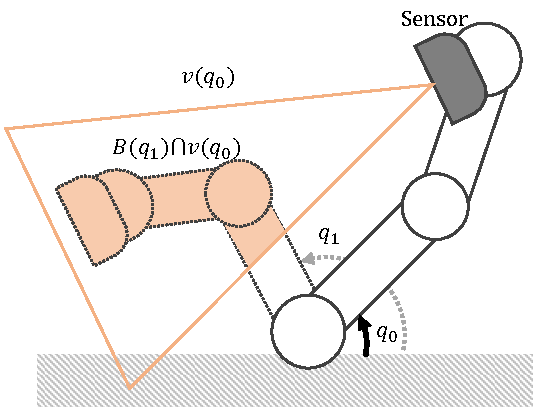
\includegraphics[width=1.0\columnwidth]{img/robot_visible.pdf}
	\caption{A three-joint 2D robot arm is shown at two configurations, $q_0$ and
	$q_1$. The robot has a sensor mounted on its end-effector. The visibility
	region of the sensor at configuration $q_0$ is shown as triangle $v(q_0)$. The
	subset of the robot's body at $q_1$ visible from $q_0$ is given by $B(q_1)
	\bigcap v(q_0)$}
	\label{fig:robot_visible}
\end{figure}

Additionally, for a configuration we can define the \textit{body} of the robot
$B_q \subseteq \R^3$, which is a set of all the points inside the robot's
links at configuration $q$ (Fig. \ref{fig:robot_visible}).  Define a trajectory
as being \textit{visible} if, for each configuration $q_i$, all of its body
points lie inside the visibility region of the trajectory from $\qinit$ to
$q_{i - 1}$ (Fig. \ref{fig:visibility}):

\begin{equation}
\vis(\xi) \Rightarrow \forall q_i \in \xi, B_{q_i} \subseteq
V_{\xi[0\ldots i - 1]}
\end{equation}

Now, the task is to find a trajectroy from $\qinit$ to $\qfinal$ which is both
\cfree, \emph{and}  \vis.

 \begin{figure}[!ht]
    \subfloat[Invalid Trajectory\label{fig:not_visible}]
    {
      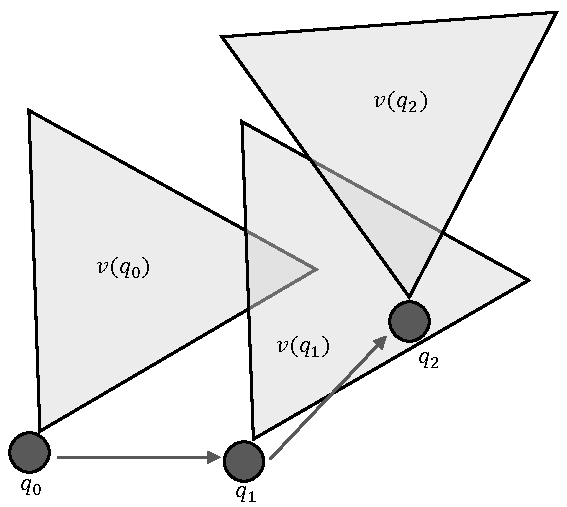
\includegraphics[width=0.46\columnwidth]{img/not_visibile.pdf}
    }
    \hfill
    \subfloat[Valid Trajectory\label{fig:visible}]
    {
      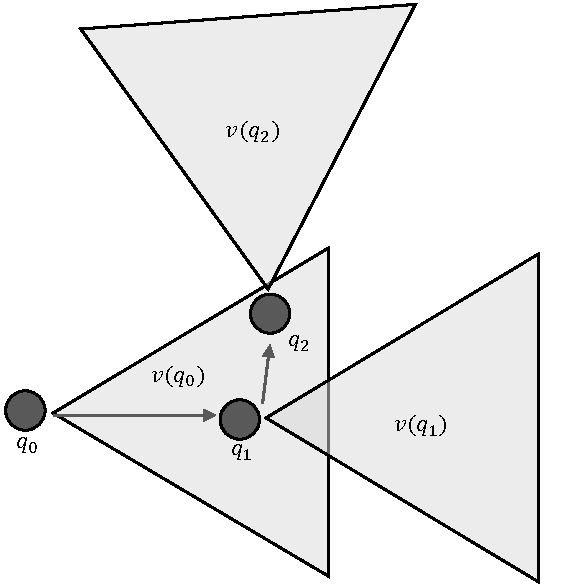
\includegraphics[width=0.46\columnwidth]{img/visible_skip}
    }
    \caption{A 2D oriented point robot with a triangular visibility region is
    shown taking two trajectories. The first trajectory (Fig.
    \ref{fig:not_visible}) violates the $\vis$ constraint, because $q_1$ is
    not in any previous configuration's visibility region. The second trajectory
    (Fig. \ref{fig:visible}) meets the $\vis$ constraint, since all the
     configurations in the trajectory are visible from some
    previous configuration}
    \label{fig:visibility}
  \end{figure}

\section{Solution Sketch}

We can solve the problem using a Rapdily Exploring Random Tree (RRT). We shall
define the RRT as a tree made up of nodes $\tau = \{n_{\text{root}}, n_1,
\ldots, n_K\}$.
Each node is a tuple $n = (q_n, p_n)$, where $q_n$ is the configuration of node $n$, and
$p_n$ is the parent node of $n$. The root node of the tree has no parent. Any
path of nodes going from parent nodes to child nodes through the tree can be
considered a trajectory. Call $\xi_n$ the trajectory from the root node of the
tree to the node $n$: 

\begin{equation}
\xi_n = \{q_{n_{\text{root}}}, \ldots, q_{p_n},  q_n\} 
\end{equation}

The basic unidirectional RRT (Alg. \ref{alg:RRT}) grows a tree from $\qinit$ to
$\qfinal$ by incrementally adding nodes to the tree while maintaining the invariant that all
trajectories through the tree from the root node at $\qinit$ to any other node
in the tree are collision-free. When $\qfinal$ in in the tree, the necessary result is a
collision-free trajectory from $\qinit$ to $\qfinal$ exists.

\begin{algorithm}
\caption{Unidirectional RRT}\label{alg:RRT}
\begin{algorithmic}[1]
\Procedure{Plan}{$\qinit, \qfinal, \text{bias}$}
   \State$\tau \gets \{(\qinit, \text{undefined})\}$
   \While{\textbf{not} $\qfinal \in \tau$}
       \State $g \gets \textsc{UniformRandom}(0, 1)$  
       \If{$g \geq \text{bias}$}
       		\State $q_r \gets \textsc{UniformRandomSample}(C)$
       \Else
       		 \State $q_r \gets \qfinal$
       \EndIf
       \State $n_n \gets \argmin_{n \in \tau} \|q_n - q_r\|$
       \State $\textsc{Extend}(n_n, q_r)$ 
   \EndWhile
   \State \textbf{return} $\xi_{n_{\text{final}}}$
\EndProcedure

\Procedure{Extend}{$\tau, n_{\text{from}}, q_{\text{to}}$}
    \State $\xi_{\text{local}}  \gets \text{LocalPlan}(q_{n_{\text{from}}},
    q_{\text{to}})$
    
    \If{$\cfree(\xi_{\text{local}})$}
         \State $\tau \gets \{\tau, (q_{\text{to}}, n_{\text{from}})\}$
    \EndIf    
\EndProcedure

\end{algorithmic}
\end{algorithm}

All we need to do is add another invariant to maintain: that all
trajectories from the root node to any other node in the tree are also
visible (Fig. \ref{fig:sphere_tree}). That is:

\begin{equation}
    \forall n \in \tau, \vis(\xi_n)
\end{equation} 

This can be achieved by modifying the \textsc{Extend} procedure so that new
nodes are added only if adding them would not break the visibility invariant
(Alg. \ref{alg:extend}).

\begin{figure}
	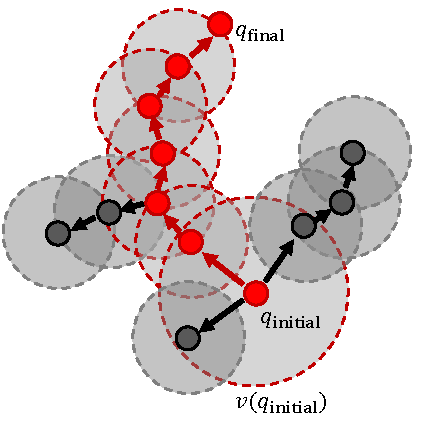
\includegraphics[width=1.0\columnwidth]{img/sphere_tree.pdf}
	\caption{An example of an RRT is shown for a point robot with a circular
	visibility region. All trajectories through the tree obey the
	$\vis$~constraint. In particular, the path from $\qinit$ to $\qfinal$ (shown in
	red) satisfies the constraint, since ever node in the path is in the visibility
	region of at least one previous node.}
	\label{fig:sphere_tree}
\end{figure}

Two ways that this can be accomplished are either by rejecting extensions which
violate the invariant (\textsc{ExtendReject}), or by generating only
invariant-preserving extensions using the Shooting Method
(\textsc{ExtendShoot}). The \textsc{ExtendShoot} method is analagous to treating
the $\vis$ invariant as a non-holonomic constraint. The result is that, as the
tree grows, all trajectories from the root to other nodes are \vis.

\begin{algorithm}
\caption{Visibility Extension with Rejection or Shooting} \label{alg:extend}
\begin{algorithmic}[1]
	\Procedure{ExtendReject}{$\tau, n_{\text{from}}, q_{\text{to}}$}
	    \State {$\xi_l  \gets \text{LocalPlan}(q_{n_{\text{from}}},
	    q_{\text{to}})$}
	    \State{$\xi_r \gets \{\xi_{n_{\text{from}}},
	    \xi_{l}\}$}
	    \State{$\text{valid} \gets \vis(\xi_r)~\textbf{and}~\cfree(\xi_l)$}
	    \If{$\text{valid}$} 
	    	\State{$\tau \gets \{\tau, (q_{\text{to}}, n_{\text{from}})\}$}
	    \EndIf   
	\EndProcedure
	
	\Procedure{ExtendShoot}{$\tau, n_{\text{from}}, q_{\text{to}}, M, U$}
		   \State{$\Xi \gets \{\}$}
		    \For{$i = 1 \ldots M$}
		        \State{$u \gets \textsc{RandomControls}()$}
		        \State{$\xi_u \gets \textsc{Shoot}(q_{\text{from}}, u, U)$}
		        \State{$\xi_u \gets \textsc{TruncateVisible}(\xi_u, n_{\text{from}})$}
		    \EndFor
		    \State{$\xi^* = \argmin_{\xi \in \Xi} \min_{q \in \xi} \| q -
		    q_{\text{to}}\|$}
		    \State{$q^* = \argmin_{q \in \xi^*} \| q - q_{\text{to}} \|$}
		    \If{$\cfree(\xi^*)$}
		        	\State{$\tau \gets \{\tau, (q^*, n_{\text{from}})\}$}
		    \EndIf 
	\EndProcedure
\end{algorithmic}
\end{algorithm}  

% trigger a \newpage just before the given reference
% number - used to balance the columns on the last page
% adjust value as needed - may need to be readjusted if
% the document is modified later
%\IEEEtriggeratref{8}
% The "triggered" command can be changed if desired:
%\IEEEtriggercmd{\enlargethispage{-5in}}

% references section

% can use a bibliography generated by BibTeX as a .bbl file
% BibTeX documentation can be easily obtained at:
% http://www.ctan.org/tex-archive/biblio/bibtex/contrib/doc/
% The IEEEtran BibTeX style support page is at:
% http://www.michaelshell.org/tex/ieeetran/bibtex/
%\bibliographystyle{IEEEtran}
% argument is your BibTeX string definitions and bibliography database(s)
%\bibliography{IEEEabrv,../bib/paper}
%
% <OR> manually copy in the resultant .bbl file
% set second argument of \begin to the number of references
% (used to reserve space for the reference number labels box)

% that's all folks
\end{document}


